\subsection{Chain of Responsibility}
\subsubsection{Định nghĩa}
Chain of Responsibility là một mẫu thiết kế hành vi (behavioral design pattern) trong lập trình, nó cho phép một loạt các đối tượng xử lý một yêu cầu tuần tự. Yêu cầu được chuyển tiếp qua các đối tượng cho đến khi có một đối tượng trong chuỗi có thể xử lý yêu cầu đó hoặc khi không còn đối tượng nào có thể xử lý.
\subsubsection{Cách sử dụng}
Thông thương ở một số trường hợp sau ta hay sử dụng chain of responsibility:
\begin{itemize}
    \item Có nhiều hơn một đối tượng có khả thực xử lý một yêu cầu trong khi đối tượng cụ thể nào xử lý yêu cầu đó lại phụ thuộc vào ngữ cảnh sử dụng.
    \item Khi có nhiều đối tượng có thể xử lý một yêu cầu và bạn muốn cho phép các đối tượng này tự động chọn đối tượng xử lý thích hợp.
    \item Khi bạn muốn tạo ra một chuỗi linh hoạt và có thể thay đổi cấu trúc xử lý yêu cầu một cách động.
\end{itemize}
\subsubsection{Cấu trúc}
\begin{center}
    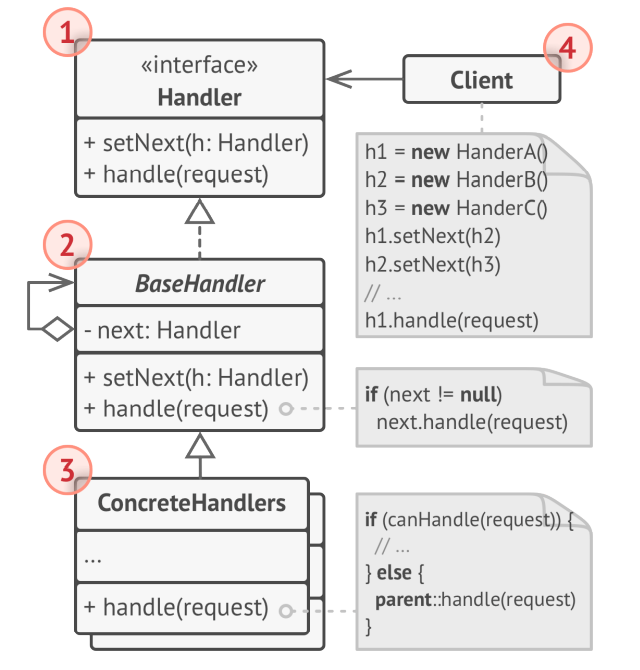
\includegraphics[scale= 0.45]{image/behavioral/cor.png}
\end{center}
\begin{itemize}
    \item Về cơ bản, cấu trúc này liên kết các class lại với nhau theo kiểu danh sách liên kết mỗi class này đều có hàm giải quyết vấn đề riêng của nó.
    \item Client sẽ sắp xếp thứ tự duyệt qua của các handlers.
\end{itemize}
Các thành phần chính:
\begin{itemize}
    \item Client là các dòng code ở trong main tạo ra các yêu cầu và yêu cầu đó sẽ được gửi đến các đối tượng tiếp nhận.
    \item Concrete Handler dùng để xử lí yêu cầu có con trỏ qua Concrete Handler khác nếu nó khong xử lí được.
    \item Handler là một interface hoặc abstract class có biến next.
    \item BaseHandler là một abstract class không bắt buộc có thể cài đặt các hàm chung cho chain of responsibility ở đây.
\end{itemize}
\subsubsection{Ưu điểm và Nhược điểm}
Ta có thể thấy tồn tại vài ưu nhược điểm sau
Ưu điểm:
\begin{itemize}
    \item Thay vì một đối tượng có khả năng xử lý yêu cầu chứa tham chiếu đến tất cả các đối tượng khác, nó chỉ cần một tham chiếu đến đối tượng tiếp theo. Tránh sự liên kết trực tiếp giữa đối tượng gửi yêu cầu (sender) và các đối tượng nhận yêu cầu (receivers).
    \item Dễ dàng thêm hoặc loại bỏ các bước xử lý trong chuỗi mà không ảnh hưởng đến các đối tượng khác.
\end{itemize}
Nhược điểm:
\begin{itemize}
    \item Một số yêu cầu có thể không được xử lý: Trường hợp tất cả Handler đều không xử lý
\end{itemize}
\subsubsection{Code Example}
\begin{itemize}
    \item Ta có một class Yêu cầu nâng cấp.
    \item Một loạt các class giải quyết yêu cầu nâng cấp có con trỏ chỉ đến bộ hanlder tiếp theo.
\end{itemize}
\begin{lstlisting}
#include <iostream>
#include <string>

class UpgradeRequest {
private:
    std::string component;
    std::string version;

public:
    UpgradeRequest(const std::string& component, const std::string& version)
        : component(component), version(version) {}

    std::string getComponent() const {
        return component;
    }

    std::string getVersion() const {
        return version;
    }
};

class UpgradeHandler {
protected:
    UpgradeHandler* nextHandler;

public:
    virtual void setNextHandler(UpgradeHandler* handler) {
        nextHandler = handler;
    }

    virtual void handleRequest(const UpgradeRequest& request) = 0;
};

class UIUpgradeHandler : public UpgradeHandler {
public:
    void handleRequest(const UpgradeRequest& request) override {
        if (request.getComponent() == "UI" && request.getVersion() == "2.0") {
            std::cout << "Upgrading UI component to version 2.0" << std::endl;
        } else if (nextHandler != nullptr) {
            nextHandler->handleRequest(request);
        } else {
            std::cout << "Upgrade request cannot be handled" << std::endl;
        }
    }
};

class DataUpgradeHandler : public UpgradeHandler {
public:
    void handleRequest(const UpgradeRequest& request) override {
        if (request.getComponent() == "Data" && request.getVersion() == "1.5") {
            std::cout << "Upgrading Data component to version 1.5" << std::endl;
        } else if (nextHandler != nullptr) {
            nextHandler->handleRequest(request);
        } else {
            std::cout << "Upgrade request cannot be handled" << std::endl;
        }
    }
};

class SecurityUpgradeHandler : public UpgradeHandler {
public:
    void handleRequest(const UpgradeRequest& request) override {
        if (request.getComponent() == "Security" && request.getVersion() == "3.2") {
            std::cout << "Upgrading Security component to version 3.2" << std::endl;
        } else if (nextHandler != nullptr) {
            nextHandler->handleRequest(request);
        } else {
            std::cout << "Upgrade request cannot be handled" << std::endl;
        }
    }
};

int main() {
    UpgradeHandler* uiUpgradeHandler = new UIUpgradeHandler();
    UpgradeHandler* dataUpgradeHandler = new DataUpgradeHandler();
    UpgradeHandler* securityUpgradeHandler = new SecurityUpgradeHandler();

    uiUpgradeHandler->setNextHandler(dataUpgradeHandler);
    dataUpgradeHandler->setNextHandler(securityUpgradeHandler);

    UpgradeRequest requestA("UI", "2.0");
    UpgradeRequest requestB("Data", "1.5");
    UpgradeRequest requestC("Security", "3.2");
    UpgradeRequest requestD("UI", "1.5");

    uiUpgradeHandler->handleRequest(requestA);
    uiUpgradeHandler->handleRequest(requestB);
    uiUpgradeHandler->handleRequest(requestC);
    uiUpgradeHandler->handleRequest(requestD);

    delete uiUpgradeHandler;
    delete dataUpgradeHandler;
    delete securityUpgradeHandler;

    return 0;
}

\end{lstlisting}
Ở hàm main, ta liên kết 3 hanlders lại với nhau. Ta có 4 yêu cầu từ khách hàng. Sau đó thực hiện giải quyết thì chỉ có duy nhất yêu cầu cuối cùng là không có bất cứ handler nào có thể giải quyết.\\
\newline
\textbf{Kết quả:}
\begin{lstlisting}
Upgrading UI component to version 2.0
Upgrading Data component to version 1.5
Upgrading Security component to version 3.2
Upgrade request cannot be handled
\end{lstlisting}
\subsubsection{Các Pattern liên quan}
\begin{itemize}
    \item Composite có thể được tích hợp chung. Ở trường hợp này các Leaf của CoR khi nhận yêu cầu sẽ được thực hiện tuần tự cho đến khi kết thúc.
    \item Có thể kết hợp với Command với các class Commands là các node lá của CoR và các command này sẽ được duyệt qua.
    \item Có thể kết hợp với Decorator bằng cách thêm thông tin vào các Leaf của CoR.
\end{itemize}
